In this section we are going to present the strategy that the development team should follow to implement \projectname~system. As we can see in the Component Dependency Diagram all the system's components have been designed in such a way that they have the least amount of dependencies, and for this reason a lot of them can be developed in parallel. In fact, all the components that are in the same column of the graph can be easily implemented by different teams. Following this process, every time that a component needs an interface from another one, that one should have been already implemented. However, this development strategy would lead to build a testable system only at the end, like in a Waterfall model, because the Meeting Controller component, that is the one of the core components of the system, would be implemented almost at the end of the process. Since modern implementation strategies are based on mid-term versions of the system, that can be shown to stakeholders, it would be very limiting to adopt this model because it will not build any prototype (e.g. alpha and beta versions) until the end of the process, denying the possibility of corrections and modifications on the go. \\
For this reasons we propose the following plan to implement the \projectname~project:
\begin{enumerate}
	
	\item Implement the Constraint Engine, the External Shortest Path Adapter and the Break Manager in parallel in order to have a solid foundation for the development of the other components.
	\item Implement the Travel Planner component.
	\item Integrate the Travel Planner with the Constraint Engine and the External Shortest Path Adapter.
	 \item[ ]
	\textbf{At this point the system should be able to find the best travel between pairs of locations. subject to given constraints.}
	 \item Implement Meeting Scheduler component. 
	 \item Integrate the Meeting Scheduler with the Travel Planner component.
	 \item[ ]
	\textbf{At this point the system should be able to properly build and update schedules.}
	 \item Implement the Meeting Controller component. Since it has still some unsolved dependencies, we will use stubs to simulate the behaviour of all the component that are not been developed yet. We will do this to be able to reach a point in which the core of the system is testable sooner.
	 \item Integrate the Meeting Controller with the Meeting Scheduler.
	 \item[ ]
	\textbf{At this point the main functionality of the system (i.e. create meeting to organize daily schedule) should be completed.}
	 \item Implement the External Login Adapter and the Authentication Engine integrating them together.
	 \item Implement the User Search Engine.
	 \item Integrate the User Search Engine with the Meeting Controller component.
	 \item Implement User Controller.
	 \item Integrate the User Controller with the User Search Engine, the Constraint Engine and the Authentication Engine.
	 \item[ ]
	\textbf{At this point a user should be able to use out system.}
	 \item Implement Rescheduling Engine and integrate it with Meeting Controller.
	 \item Implement Notification Engine and integrate it with the Meeting Controller and the Rescheduling Engine.
	 \item[ ]
	\textbf{At this point a Beta version could be shipped.}
	 \item Implement the File Uploader, the Chat Engine and the Late User Engine in parallel.
	 \item Integrate the File Uploader, the Chat Engine and the Late User Engine with the Meeting Controller, replacing the previously inserted stubs.
	 \item Implement the External Geolocalization Adaper and the Real-Time Indications Engine integrating them together.
	 \item[ ]
	\textbf{At this point the first working version of \projectname~can be considered completed.}
\end{enumerate}

\begin{figure}[!h]
	\centering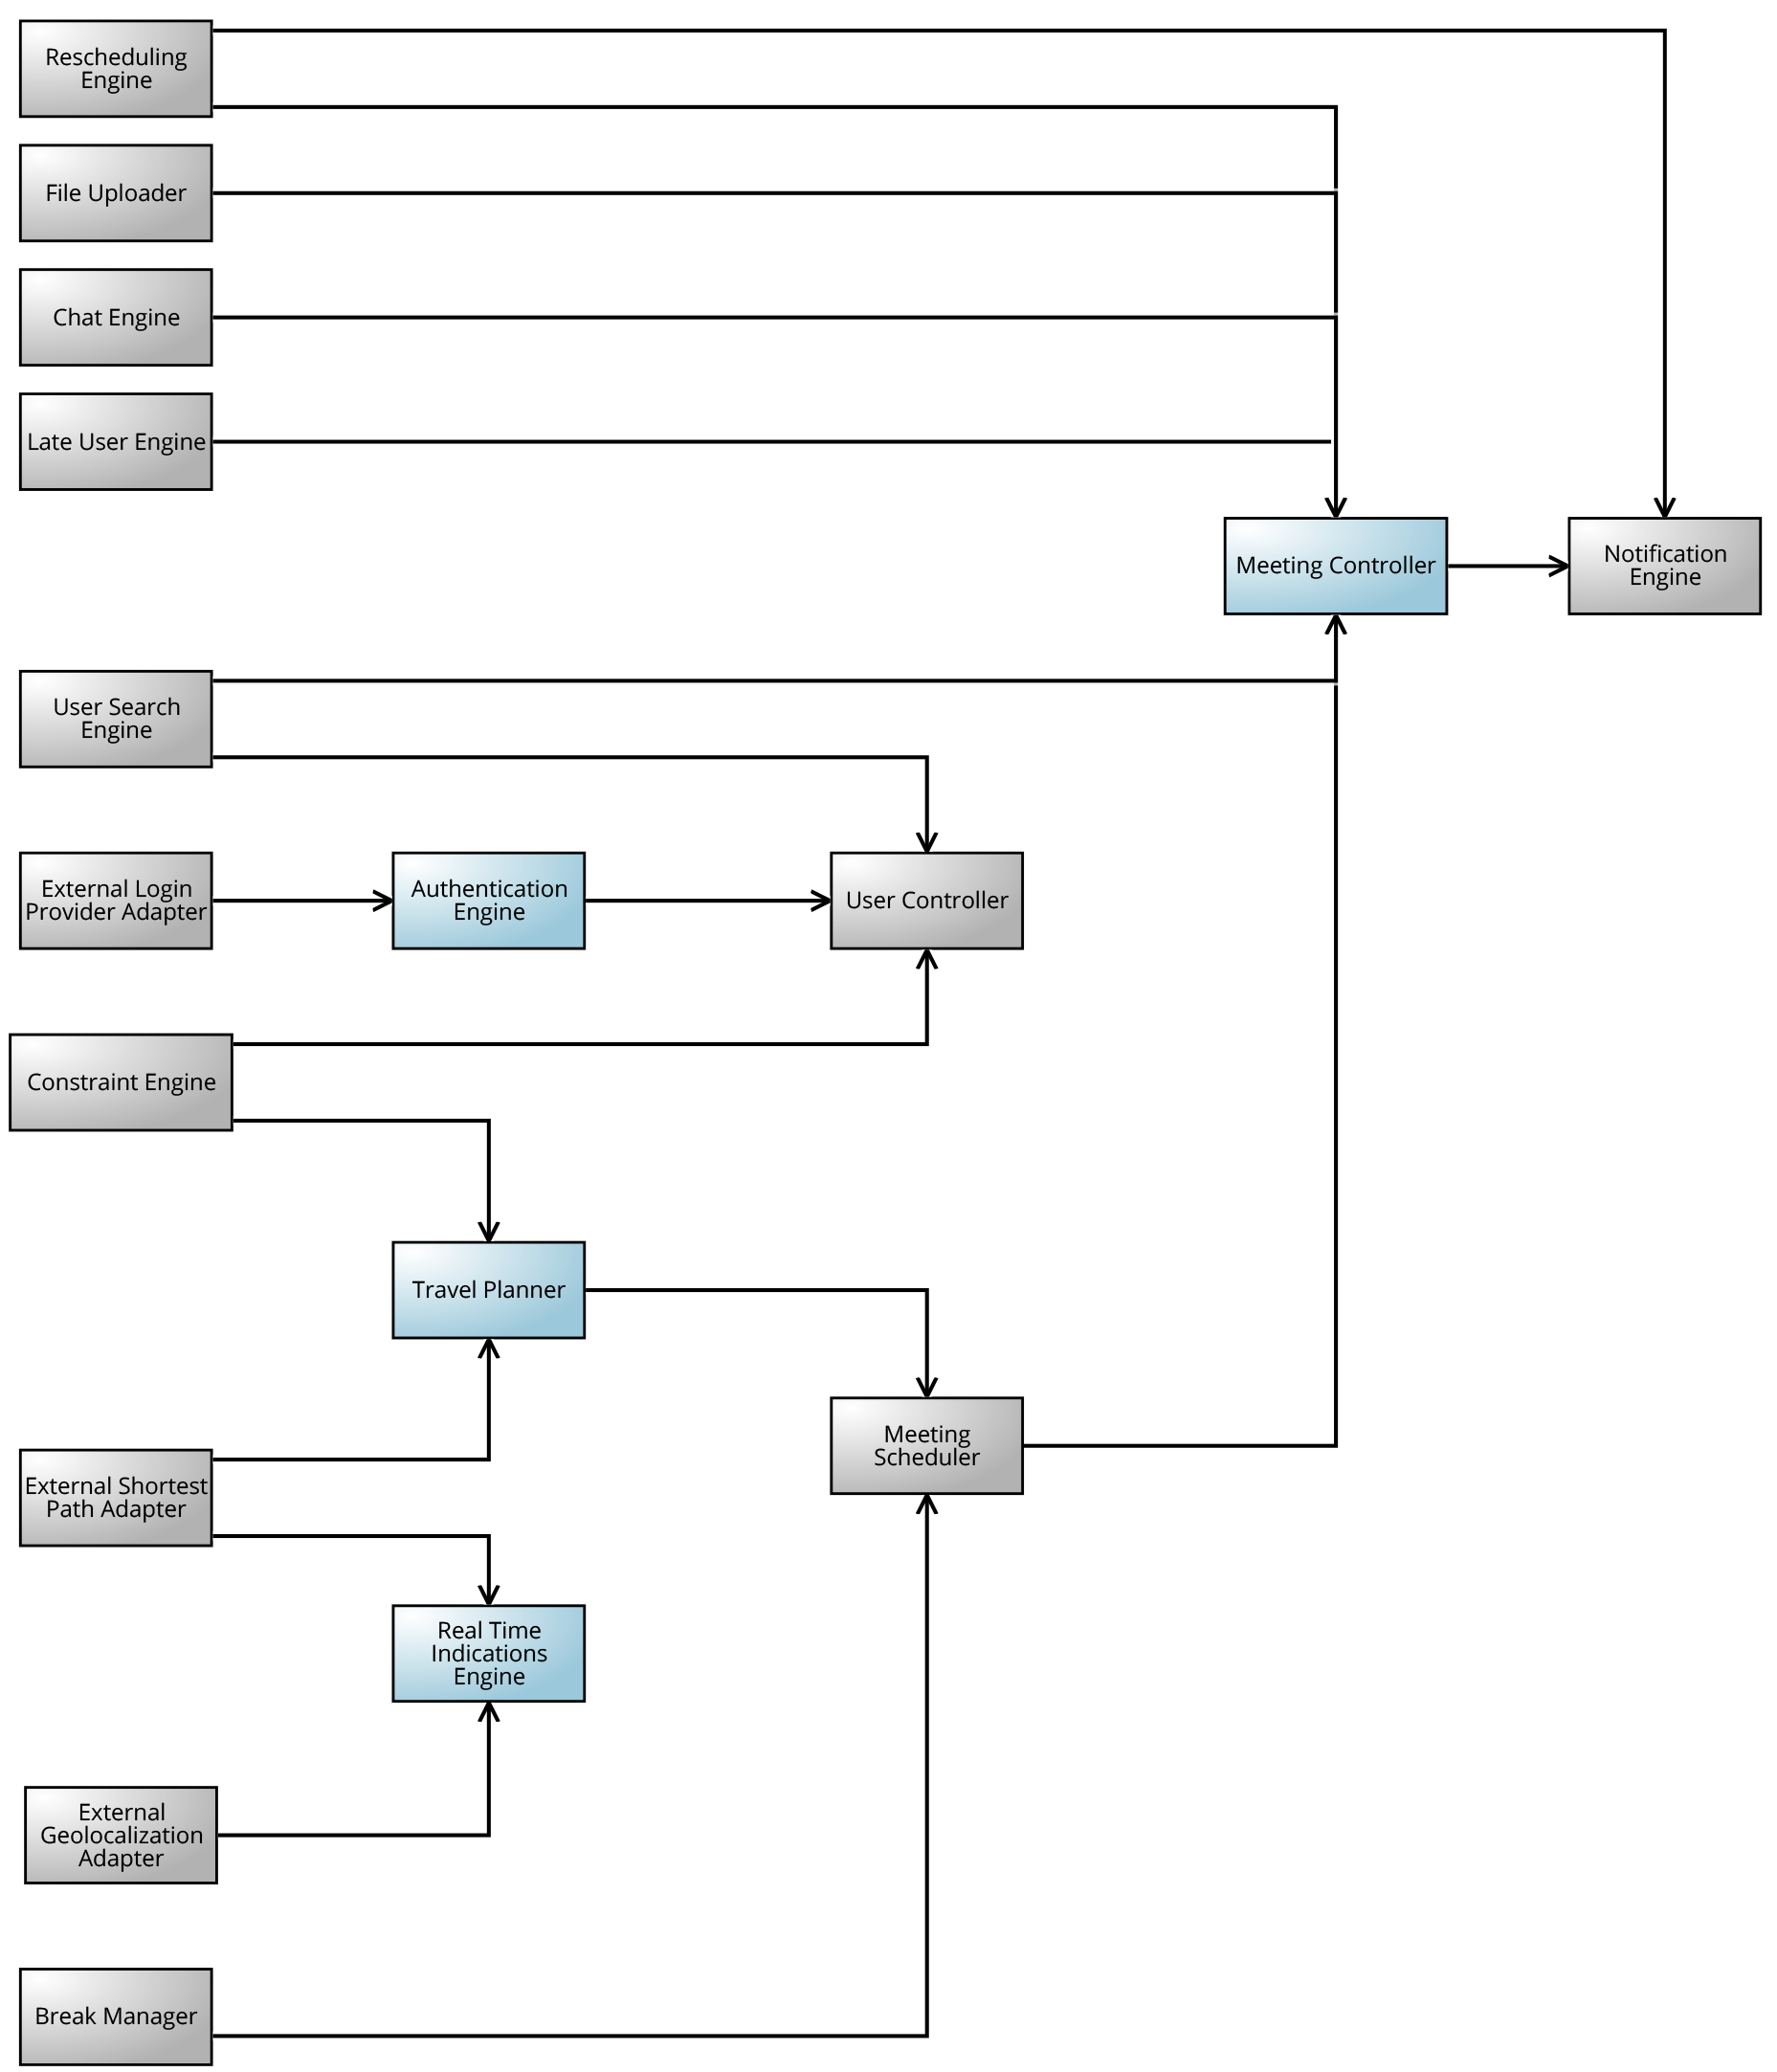
\includegraphics[scale = 0.19]{Images/UMLDiagrams/DependencyDiagramColored.png}
	\caption{Component Dependency Diagram}
\end{figure}

\clearpage